\title{Warm-Up for April 1st, 2022}
\author{Dr. Jordan Hanson - Whittier College Dept. of Physics and Astronomy}
\date{\today}
\documentclass[12pt]{article}
\usepackage[a4paper, total={18cm, 27cm}]{geometry}
\usepackage{graphicx}
\usepackage{amsmath}
\usepackage{bm}
\def\rcurs{{\mbox{$\resizebox{.16in}{.08in}{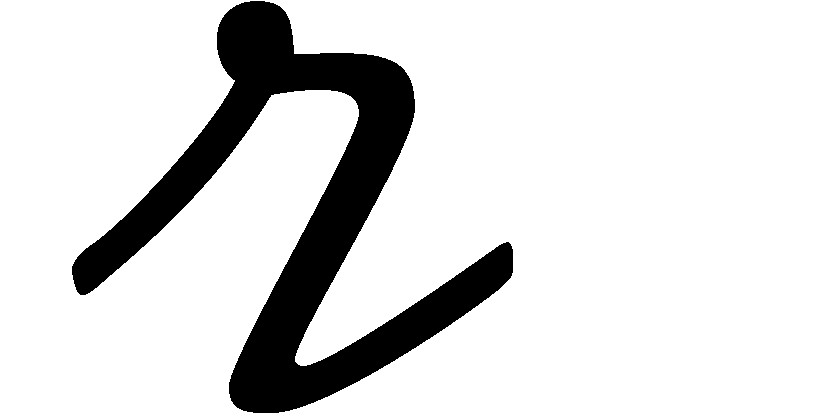
\includegraphics{ScriptR}}$}}}
\def\brcurs{{\mbox{$\resizebox{.16in}{.08in}{
\includegraphics{BoldR}}$}}}
\def\hrcurs{{\mbox{$\hat \brcurs$}}}
 
\begin{document}
\small
\maketitle
\small
\section{Memory Bank}
\begin{enumerate}
\item The electric displacement ... $\mathbf{D} = \epsilon_0 \mathbf{E} + \mathbf{P}$
\item Gauss' Law for displacement ... $\nabla \cdot \mathbf{D} = \rho_f$, $\oint \mathbf{D} \cdot d\mathbf{a} = Q_{\rm f,enc}$
\item For a linear dielectric ... $\mathbf{P} = \epsilon_0 \chi_e \mathbf{E}$, \hspace{0.25cm} $\mathbf{D} = \epsilon_0(1+\chi_e) \mathbf{E} = \epsilon \mathbf{E}$
\item Relative permittivity/dielectric constant ... $\epsilon_r = 1+\chi_e = \epsilon/\epsilon_0$
\item Speed of an electromagnetic plane wave in a linear dielectric ... $v = c/n$, where $c$ is the speed of light and $n = \sqrt{\epsilon_r}$.
\end{enumerate}

\section{Linear Dielectrics}

\begin{enumerate}
\item The space between the plates of a parallel-plate capacitor (Fig. \ref{fig:1}) is filled with two slabs of linear dielectric material.  Each slab has thickness $a$, so the total distance between plates is $2a$.  Slab 1 has a dielectric constant of 2, and slab 2 has a dielectric constant of 1.5.  The free charge density on the top plate is $\sigma$ and on the bottom plate $-\sigma$.
\begin{itemize}
\item (a) Find $\mathbf{D}$ in each slab.
\item (b) Find $\mathbf{E}$ in each slab.
\item (c) Find $\mathbf{P}$ in each slab.
\item (d) Find $\Delta V$ between the plates.
\end{itemize}
\end{enumerate}

\begin{figure}
\centering
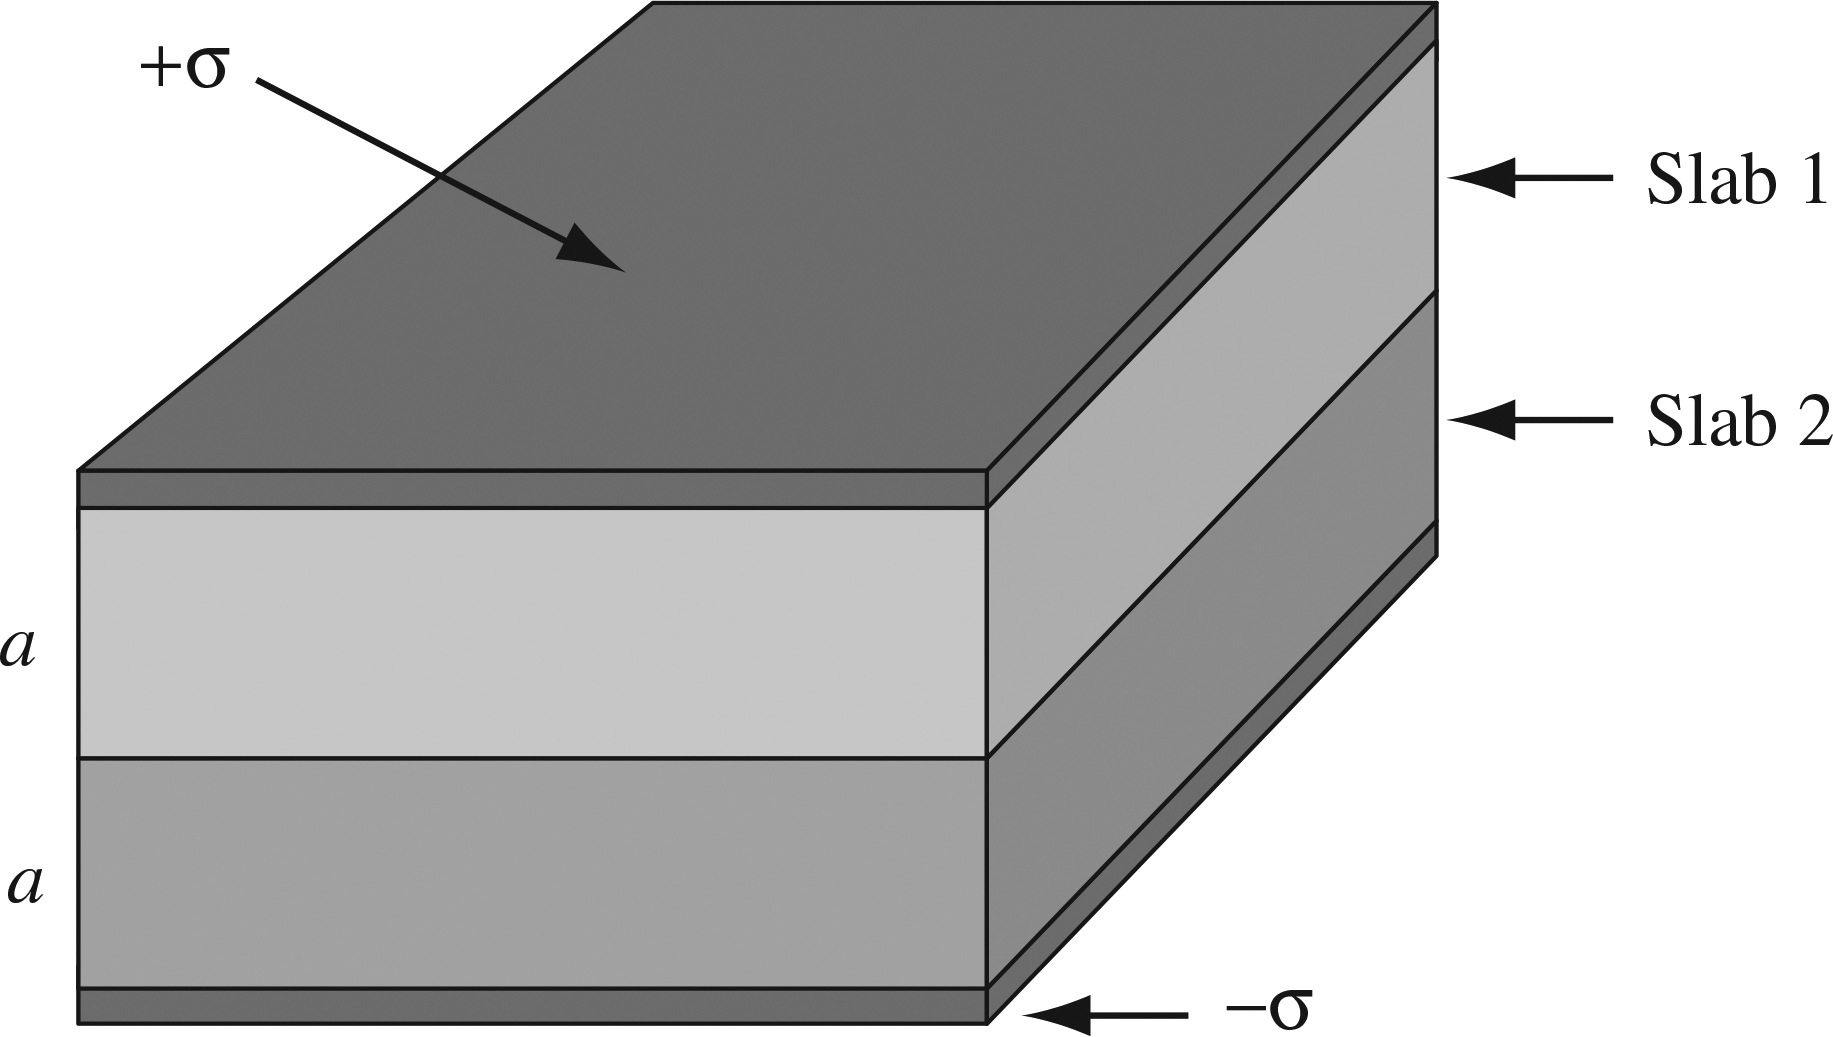
\includegraphics[width=0.4\textwidth]{figures/4_24.jpg}
\caption{\label{fig:1} A capacitor with some linear dielectric in between the plates.}
\end{figure}

\end{document}